


\tikzset{every picture/.style={line width=0.75pt}} %set default line width to 0.75pt        

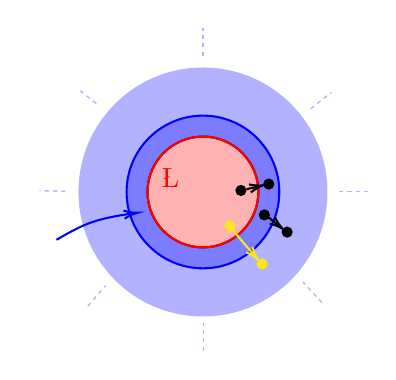
\begin{tikzpicture}[x=0.75pt,y=0.75pt,yscale=-1,xscale=1,scale=0.6]
%uncomment if require: \path (0,893); %set diagram left start at 0, and has height of 893

%Shape: Circle [id:dp6347747926336691] 
\draw  [draw opacity=0][fill={rgb, 255:red, 0; green, 0; blue, 255 }  ,fill opacity=0.3 ] (185.73,741.1) .. controls (185.73,685.89) and (230.49,641.13) .. (285.7,641.13) .. controls (340.91,641.13) and (385.67,685.89) .. (385.67,741.1) .. controls (385.67,796.31) and (340.91,841.07) .. (285.7,841.07) .. controls (230.49,841.07) and (185.73,796.31) .. (185.73,741.1) -- cycle ;
%Shape: Circle [id:dp16773685093033808] 
\onslide<10->{\draw  [color={rgb, 255:red, 0; green, 0; blue, 255 }  ,draw opacity=1 ][fill={rgb, 255:red, 0; green, 0; blue, 255 }  ,fill opacity=0.3 ] (224.39,741.1) .. controls (224.39,707.24) and (251.84,679.79) .. (285.7,679.79) .. controls (319.56,679.79) and (347.01,707.24) .. (347.01,741.1) .. controls (347.01,774.96) and (319.56,802.41) .. (285.7,802.41) .. controls (251.84,802.41) and (224.39,774.96) .. (224.39,741.1) -- cycle ;}
%Shape: Circle [id:dp86831620873002] 
\draw  [fill={rgb, 255:red, 255; green, 255; blue, 255 }  ,fill opacity=1 ] (241.2,741.1) .. controls (241.2,716.52) and (261.12,696.6) .. (285.7,696.6) .. controls (310.28,696.6) and (330.2,716.52) .. (330.2,741.1) .. controls (330.2,765.68) and (310.28,785.6) .. (285.7,785.6) .. controls (261.12,785.6) and (241.2,765.68) .. (241.2,741.1) -- cycle ;
%Shape: Circle [id:dp09468292282767443] 
\draw  [color={rgb, 255:red, 255; green, 0; blue, 0 }  ,draw opacity=1 ][fill={rgb, 255:red, 255; green, 0; blue, 0 }  ,fill opacity=0.3 ] (241.2,741.1) .. controls (241.2,716.52) and (261.12,696.6) .. (285.7,696.6) .. controls (310.28,696.6) and (330.2,716.52) .. (330.2,741.1) .. controls (330.2,765.68) and (310.28,785.6) .. (285.7,785.6) .. controls (261.12,785.6) and (241.2,765.68) .. (241.2,741.1) -- cycle ;
%Shape: Circle [id:dp9845956832929754] 
\draw  [draw opacity=0][fill={rgb, 255:red, 0; green, 0; blue, 0 }  ,fill opacity=1 ][line width=0.75]  (311.7,739.9) .. controls (311.7,737.41) and (313.71,735.4) .. (316.2,735.4) .. controls (318.69,735.4) and (320.7,737.41) .. (320.7,739.9) .. controls (320.7,742.39) and (318.69,744.4) .. (316.2,744.4) .. controls (313.71,744.4) and (311.7,742.39) .. (311.7,739.9) -- cycle ;
%Shape: Circle [id:dp7570400850625347] 
\draw  [draw opacity=0][fill={rgb, 255:red, 0; green, 0; blue, 0 }  ,fill opacity=1 ][line width=0.75]  (334.07,734.73) .. controls (334.07,732.25) and (336.08,730.23) .. (338.57,730.23) .. controls (341.05,730.23) and (343.07,732.25) .. (343.07,734.73) .. controls (343.07,737.22) and (341.05,739.23) .. (338.57,739.23) .. controls (336.08,739.23) and (334.07,737.22) .. (334.07,734.73) -- cycle ;
%Straight Lines [id:da4946555213004382] 
\draw    (320.7,738.9) -- (332.12,736.19) ;
\draw [shift={(334.07,735.73)}, rotate = 166.67] [color={rgb, 255:red, 0; green, 0; blue, 0 }  ][line width=0.75]    (10.93,-3.29) .. controls (6.95,-1.4) and (3.31,-0.3) .. (0,0) .. controls (3.31,0.3) and (6.95,1.4) .. (10.93,3.29)   ;
\onslide<10->{%Shape: Circle [id:dp21475200286126772] 
\draw  [draw opacity=0][fill={rgb, 255:red, 0; green, 0; blue, 0 }  ,fill opacity=1 ][line width=0.75]  (330.5,759.5) .. controls (330.5,757.01) and (332.51,755) .. (335,755) .. controls (337.49,755) and (339.5,757.01) .. (339.5,759.5) .. controls (339.5,761.99) and (337.49,764) .. (335,764) .. controls (332.51,764) and (330.5,761.99) .. (330.5,759.5) -- cycle ;
%Shape: Circle [id:dp6401125405786658] 
\draw  [draw opacity=0][fill={rgb, 255:red, 0; green, 0; blue, 0 }  ,fill opacity=1 ][line width=0.75]  (348.8,773.3) .. controls (348.8,770.81) and (350.81,768.8) .. (353.3,768.8) .. controls (355.79,768.8) and (357.8,770.81) .. (357.8,773.3) .. controls (357.8,775.79) and (355.79,777.8) .. (353.3,777.8) .. controls (350.81,777.8) and (348.8,775.79) .. (348.8,773.3) -- cycle ;
%Straight Lines [id:da6137452163851853] 
\draw    (337.67,760.93) -- (348.44,769.64) ;
\draw [shift={(350,770.9)}, rotate = 218.94] [color={rgb, 255:red, 0; green, 0; blue, 0 }  ][line width=0.75]    (10.93,-3.29) .. controls (6.95,-1.4) and (3.31,-0.3) .. (0,0) .. controls (3.31,0.3) and (6.95,1.4) .. (10.93,3.29)   ;}
%Shape: Circle [id:dp4856749631522035] 
\onslide<11->{\draw  [draw opacity=0][fill={rgb, 255:red, 248; green, 231; blue, 28 }  ,fill opacity=1 ][line width=0.75]  (302.9,768.5) .. controls (302.9,766.01) and (304.91,764) .. (307.4,764) .. controls (309.89,764) and (311.9,766.01) .. (311.9,768.5) .. controls (311.9,770.99) and (309.89,773) .. (307.4,773) .. controls (304.91,773) and (302.9,770.99) .. (302.9,768.5) -- cycle ;
%Shape: Circle [id:dp8734179708310015] 
\draw  [draw opacity=0][fill={rgb, 255:red, 248; green, 231; blue, 28 }  ,fill opacity=1 ][line width=0.75]  (328.8,798.9) .. controls (328.8,796.41) and (330.81,794.4) .. (333.3,794.4) .. controls (335.79,794.4) and (337.8,796.41) .. (337.8,798.9) .. controls (337.8,801.39) and (335.79,803.4) .. (333.3,803.4) .. controls (330.81,803.4) and (328.8,801.39) .. (328.8,798.9) -- cycle ;
%Straight Lines [id:da3880974951160452] 
\draw [color={rgb, 255:red, 248; green, 231; blue, 28 }  ,draw opacity=1 ][fill={rgb, 255:red, 155; green, 155; blue, 155 }  ,fill opacity=1 ]   (309.67,771.73) -- (328.77,794.21) ;
\draw [shift={(330.07,795.73)}, rotate = 229.64] [color={rgb, 255:red, 248; green, 231; blue, 28 }  ,draw opacity=1 ][line width=0.75]    (10.93,-3.29) .. controls (6.95,-1.4) and (3.31,-0.3) .. (0,0) .. controls (3.31,0.3) and (6.95,1.4) .. (10.93,3.29)   ;}
%Straight Lines [id:da5165162315025413] 
\draw [color={rgb, 255:red, 0; green, 0; blue, 255 }  ,draw opacity=0.3 ][line width=0.5]  [dash pattern={on 1.5pt off 1.5pt}]  (395.07,740.53) -- (417.87,740.53) ;
%Straight Lines [id:da38753837989284445] 
\draw [color={rgb, 255:red, 0; green, 0; blue, 255 }  ,draw opacity=0.3 ][line width=0.5]  [dash pattern={on 1.5pt off 1.5pt}]  (372.27,674.33) -- (388.67,661.13) ;
%Straight Lines [id:da007919123820054441] 
\draw [color={rgb, 255:red, 0; green, 0; blue, 255 }  ,draw opacity=0.3 ][line width=0.5]  [dash pattern={on 1.5pt off 1.5pt}]  (285.67,631.73) -- (285.67,609.73) ;
%Straight Lines [id:da7968663560498248] 
\draw [color={rgb, 255:red, 0; green, 0; blue, 255 }  ,draw opacity=0.3 ][line width=0.5]  [dash pattern={on 1.5pt off 1.5pt}]  (200.07,670.13) -- (184.47,657.73) ;
%Straight Lines [id:da48757360196126287] 
\draw [color={rgb, 255:red, 0; green, 0; blue, 255 }  ,draw opacity=0.3 ][line width=0.5]  [dash pattern={on 1.5pt off 1.5pt}]  (175.27,740.53) -- (154.47,740.13) ;
%Straight Lines [id:da11971479686666275] 
\draw [color={rgb, 255:red, 0; green, 0; blue, 255 }  ,draw opacity=0.3 ][line width=0.5]  [dash pattern={on 1.5pt off 1.5pt}]  (286.07,868.53) -- (286.07,846.53) ;
%Straight Lines [id:da6484236736378048] 
\draw [color={rgb, 255:red, 0; green, 0; blue, 255 }  ,draw opacity=0.3 ][line width=0.5]  [dash pattern={on 1.5pt off 1.5pt}]  (381.27,829.88) -- (366.07,813.39) ;
%Straight Lines [id:da25336093141802474] 
\draw [color={rgb, 255:red, 0; green, 0; blue, 255 }  ,draw opacity=0.3 ][line width=0.5]  [dash pattern={on 1.5pt off 1.5pt}]  (193.27,832.68) -- (207.67,816.19) ;
%Curve Lines [id:da46026392802664984] 
\onslide<10->{\draw [color={rgb, 255:red, 0; green, 0; blue, 255 }  ,draw opacity=1 ]   (168.07,779.48) .. controls (190.92,766.47) and (197.86,762.79) .. (231.61,757.97) ;
\draw [shift={(233.17,757.75)}, rotate = 172.01] [color={rgb, 255:red, 0; green, 0; blue, 255 }  ,draw opacity=1 ][line width=0.75]    (10.93,-3.29) .. controls (6.95,-1.4) and (3.31,-0.3) .. (0,0) .. controls (3.31,0.3) and (6.95,1.4) .. (10.93,3.29)   ;}

% Text Node
\draw (250.2,719.6) node [anchor=north west][inner sep=0.75pt]  [color={rgb, 255:red, 255; green, 0; blue, 0 }  ,opacity=1 ]  {$\L$};
% Text Node
\onslide<10->{\draw (145.8,774) node [anchor=north west][inner sep=0.75pt]  [color={rgb, 255:red, 0; green, 0; blue, 255 }  ,opacity=1 ]  {$\U$};}


\end{tikzpicture}
